
data model:
2D geometries
no self intersection
clean geometries
allow to be non-exhaustive (have holes e.g. enclaves, exclaves)
rules of simple polygon (look @ wikipedia)

feature topology table
points          ID, coordinates
polylines       ID, [points]        no direction, all splines order 1
polygons        ID, [polylines]
polypolygons    ID, [polygons]      account for islands
--> concept of ``multiaffilation''

interior border: discrete phenomenon
coastline: continuous phenomenon
-> combined for whole country border
-> have to deal with both

idea: strict connectivity -> topological network

modeling historical border changes


% - - - - - - - - - - - - - - - - - - - - - - - - - - - - - - - - - - - - - - -
\paragraph{Pseudocode description} % (fold)
\label{par:pseudocode_description}

of the HG operations in an object-oriented manner. The existance of a class \texttt{Area} is assumed. Each \texttt{Area} object has the following member variables: a \texttt{name}, a \texttt{territory} and a list of historical \texttt{predecessors} and \texttt{successors}. Single capital letter variables (\texttt{A}/\texttt{B}) denote arrays of \texttt{Area} objects. Variables with a capital letter followed by a number or lowercase letter (e.g. \texttt{B0}) are single \texttt{Area} objects.

\begin{minipage}[t]{0.47\textwidth}
\begin{lstlisting}[language=pseudocode,
  caption=Unification]
FUNCTION UNI(A, B0_name)
  # create new territory
  B0_territory = NEW Geometry # empty
  FOREACH Ai IN A
    B0_territory.union(Ai.territory)
  # create new area
  B0 = NEW Area(B0_name, B0_territory)
  # establish historical relationships
  FOREACH Ai IN A
    Ai.successors.add(B0)
    B0.predecessors.add(A1)
  # return new area
  RETURN B0
\end{lstlisting}
\end{minipage}    % N.B. the % is very important
\hspace{3.0em}    % N.B. this must go in this line, no blank lines !!!
\begin{minipage}[t]{0.47\textwidth}
\begin{lstlisting}[language=pseudocode,
  caption=Incorporation]
FUNCTION INC(A0, A)
  # update old area with new territory
  temp_terr = NEW Geometry # empty
  FOREACH Ai IN A
    temp_terr.union(Ai.territory)
  A0.territory = temp_terr
  # establish historical relationships
  FOREACH Ai IN A
    Ai.successor.add(A0)
    A0.predecessor.add(A1)
  # return new area
  RETURN A0
\end{lstlisting}
\end{minipage}

\begin{minipage}[t]{0.47\textwidth}
\begin{lstlisting}[language=pseudocode,
  caption=Separation]
FUNCTION SEP(A0, B_data)
  # create each new Area
  B = []
  FOREACH Bi_data in B_data
    B.add(NEW Area(
      Bi_data.name, Bi_data.territory)
    )
  # establish historical relationships
  FOREACH Bi IN B
    A0.successors.add(Bi)
    Bi.predecessors.add(A0)
  # return new areas
  RETURN B

\end{lstlisting}
\end{minipage}    % N.B. the % is very important
\hspace{3.5em}    % N.B. this must go in this line, no blank lines !!!
\begin{minipage}[t]{0.47\textwidth}
\begin{lstlisting}[language=pseudocode,
  caption=Secession]
FUNCTION SEC(A0, A_territory, B_data)
  # update old area with new territory
  A0.territory = A_territory
  # create each new Area
  B = []
  FOREACH Bi_data in B_data
    B.add(NEW Area(
      Bi_data.name, Bi_data.territory)
    )
  # establish historical relationships
  FOREACH Bi IN B
    A0.successors.add(Bi)
    Bi.predecessors.add(A0)
  # return old and new areas
  RETURN [A0, B]

\end{lstlisting}
\end{minipage}

\vspace{-1.5em}
\begin{minipage}[t]{0.47\textwidth}
\begin{lstlisting}[language=pseudocode,
  caption=Name Change]
FUNCTION NCH(A0, A_name)
  # update old area with new name
  A0.name = A_name
  # return updated area
  RETURN A0

\end{lstlisting}
\end{minipage}

% paragraph pseudocode_description (end)


\paragraph{Execute Historical Change} % (fold)
\label{par:execute_historical_change}

execute function for all operations the same

% - - - - - - - - - - - - - - - - - - - - - - - - - - - - - - - - - - - - - - -
\begin{lstlisting}[language=pseudocode,
  caption=class HGOperation]
## member variables
old_areas = []          # Area
new_areas = []          # Area
update_name = {
  area :          null  # Area
  old_name :      null  # AreaName
  new_name :      null  # AreaName
}
update_territory = {
  area :          null  # Area
  old_territory : null  # AreaTerritory
  new_territory : null  # AreaTerritory
}

## main function
FUNCTION execute(direction)

  # hide old areas
  FOREACH old_area IN old_areas
    IF direction IS 1 # forward change
      old_area.hide()
    ELSE              # backward change
      old_area.show()

  # show new areas
  FOREACH new_area IN new_areas
    IF direction IS 1 # forward change
      new_area.show()
    ELSE              # backward change
      new_area.hide()

  # check if the area name is updated
  IF update_name.area
    IF direction IS 1 # forward change
      update_name.area.name = new_name
    ELSE              # backward change
      update_name.area.name = old_name
    update_name.area.update()

  # check if the area territory is updated
  IF update_territory.area
    IF direction IS 1 # forward change
      update_territory.area.territory = new_territory
    ELSE              # backward change
      update_territory.area.territory = old_territory

\end{lstlisting}

% paragraph execute_historical_change (end)

HistoGraph
\begin{lstlisting}[language=pseudocode,
  caption=plotting Areas on the HistoGraph,
  label=lst:histograph_plot]
FUNCTION plot(reference_area, plot_start_date, plot_end_date)
  # plot the current Area
  # logic is omitted

  # recursively plot in historically backward direction
  FOREACH predecessor IN reference_area.predecessors
    IF predecessor.end_date >= plot_start_date
      plot(predecessor)

  # recursively plot in historically forward direction
  FOREACH successor IN reference_area.successors
    IF successor.start_date <= plot_end_date
      plot(successor)
\end{lstlisting}

store Hivents in DoublyLinkedList

% \begin{figure}[ht]
%   \centering
%   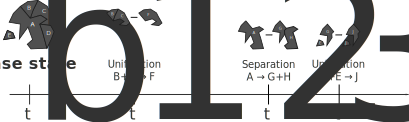
\includegraphics[width=0.8\textwidth]{graphics/basics/stdm/event-based_spatio-temporal_data_model}
%   \caption{The Event-Based Spatio-Temporal Data Model}
%   \label{fig:event-based_spatio-temporal_data_model}

% % - - - - - - - - - - - - - - - - - - - - - - - - - - - - - - - - - - - - - - -
% \paragraph{Functional description} % (fold)
% \label{par:functional_description}

% Each Hivent Operation can be described by a mathematical function. The following symbols are used in the equations:

% \begin{addmargin}[1em]{0em}
% \begin{tabbing}
%   symbolxx \= description1xx \= description2 \kill
%   $A$ \> set of old Areas that were active before the Historical Change \\
%   $B$ \> set of new Areas that are created in the Historical Change \\
%   $n:$ \> $n \in \mathbb{N}, n>0$ \> total number of old respectively new Areas \\
%   $i:$ \> $i \in [\textbf{1} .. n]$ \> iterator for the current old respectively new Area \\
%   $A_0/B_0$ \>    the first old respectively new Area ($i \geq 1 \Rightarrow$ not $A_i/B_i$~!) \\
%   $A_i/B_i$ \>    the current old respectively new Area ($i \geq 1 \Rightarrow$ not $A_0/B_0$~!) \\
%   $A_i^T/B_i^T$ \>the new territory of the current Area (a polypolygon) \\
%   $A_i^N/B_i^N$ \>the new name of the current Area (short and formal name) \\
% \end{tabbing}
% \end{addmargin}

% \vspace{-2.5em}
% \begin{align*}
%   (B_0)                       &= UNI([A_1 .. A_i .. A_n], B_0^N) \\
%   (A_0)                       &= INC(A_0, [A_1 .. A_i .. A_n]) \\
%   ([B_1 .. B_i .. B_n])       &= SEP(A_0, [[B_1^T, B_1^N] .. [B_i^T, B_i^N] .. [B_n^T, B_n^N]]) \\
%   (A_0, [B_1 .. B_i .. B_n])  &= SEC(A_0, A_0^T, [[B_1^T, B_1^N] .. [B_i^T, B_i^N] .. [B_n^T, B_n^N]]) \\
%   (A_0)                       &= NCH(A_0, A_0^N)
% \end{align*}

% % paragraph functional_description (end)
